\documentclass[a4paper,12pt]{report}
\usepackage{anysize}



\usepackage{graphicx}
\usepackage{latexsym}
\usepackage{amssymb}
\usepackage{amsmath}
\usepackage{color}
\usepackage[english]{babel}
\usepackage[latin1]{inputenc}
\usepackage{fancyhdr}
%%Algorithm
\usepackage[longend,linesnumbered,boxruled,algosection,lined]{settings/algorithm2e}
\usepackage{settings/firstpage} % modificare questo file per i diplomi e se si ha
                        % un solo correlatore
\usepackage{fullpage}


%% \hyphenation{} is used to force the 
\hyphenation{}

\newtheorem{Definition}{Definition}[section]

\pagestyle{fancy}
\marginsize{2cm}{2cm}{1cm}{3cm}
\begin{document}

\title{Standard MicroLab: \LaTeX }
\providecommand{\annoacc}{2010}

% genera la prima pagina
\titlfp

%\maketitle
\titlepage



\headsep 1cm

\setlength{\headwidth}{\textwidth}
  %uncomment the following line to remove chapter in the header
  \fancyhead[R]{}

   \fancyhead[L]{
   	\includegraphics*[width=1in]{img/scritta}
   	%with this you can move up or down the title in order not to overlap with chapter title.
   	\raisebox{5mm}
   	{	
      	\begin{tabular}{l}
      		%Prova di titolo
      	\end{tabular}
   	}
	}

	\fancyfoot[C]{\thepage}
	\renewcommand{\footrulewidth}{0.4pt}

\newpage

\tableofcontents

\newpage

\listoffigures

%\newpage

%\listoftables

%============= ABSTRACT ====================
\newpage
\begin{abstract}
2 righe sul lavoro, ->VENDITI BENE
\end{abstract}


%============================= INTRODUCTION =================================
\newpage
\chapter{Project Introduction}\label{sec:intro}




%============================= SECTIONS =================================

\newpage
\chapter{Qca Overview}\label{sec:qca}

Quantum Dot Cellular Automata (QCA) are a quantum extension to the classical notion of Cellular Automata. 

In computability theory, we identify a Cellular Automata (CA) as a Turing-complete abstract machine model consisting of a grid of \textsl{cells} each of which can be in any of a finite number of \textsl{states}. For every cell in the grid, moreover, we define its \textsl{neighborhood}, which is the set of "near enough" cells. The \textsl{evolution} of this automaton is defined by the transition of the state of the cells, which is a function of both the status of the cell and the status of its neighborhood.

What makes a QCA different from a classical CA is that its physical implementation is regulated by the quantum laws of physics instead of the classical ones. Let's take a closer look to a QCA. As you can see in \figurename~\ref{fig:qca} a QCA is made of three main components: electron wells, crystalline substrate and electrons. Here we depict the charge of the electrons on the wells/dots by blurred blue clouds instead of the more classical representation of small, crisply defined points. This is accurate because the Quantum Mechanics says that at this near atomic scale, charge (on electrons and protons) does not come in sharp little balls, but instead is correctly representable only in a probabilistic way via the wave function (Schr\"{o}dinger equation).

\begin{figure}[h!bt]
	\centerline{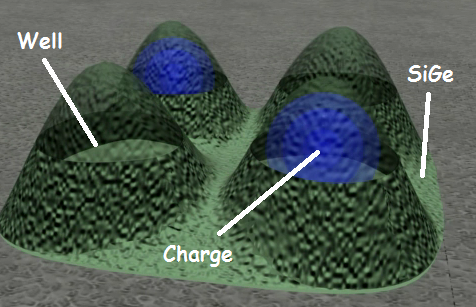
\includegraphics[width=0.9\textwidth]{img/qca.png}}
	\caption{A single Quantum Dot Cellular Automata (QCA) cell. In green the crystalline (SiGe - Silicon Germanium) substrate, where are clearly visible, in squared position, the four wells meant for accomodating that many electrons. Even though different configurations of the dots are possible, this is by far the most commonly studied structure. The blue cloud represents the amplitude of probability of finding an electron in that position.}
	\label{fig:qca}
\end{figure}

Charges of the same type (positive or negative) still repel one another so our two clouds of charge will move as far from the another as possible by moving to opposite corners of the QCA (this allows for the largest distance to be set between the clouds). In \figurename~\ref{fig:qcaevo} is represented the typical evolution of a QCA cell. What is the phenomenon that allows a charge to move from a well to the other? This is called ''tunnel effect'', a well known phenomenon in quantum physics that predicts that, under certain hypothesis, waves (in our case: the cloud) are enabled to move trespassing thin layers of obstructing materials (in our case: the walls of the wells). This is the main distinguishing reason why these cells are not simply cellular automata but quantum ones. This must not lead the reader to think that these devices, just \textsl{per se}, allow for quantum computing to take place. In fact, these devices, as for have been described, always behave in a deterministic manner, being polarized in one or the other proposed configurations. Quantum computing by means of QCA cells exploitation has been demonstrated feasible from a mathemathical point of view, but no real world implementations, to date, have publicily been demonstrated.  

The only (from a theorethical point of view) remaining feature that is required to enable the transmission of data troughut a circuit of adjacent QCA cells is the concept of ''clock''. Clocks are areas of conductive material under the circuit's lattice, modulating the electron tunneling barriers in the QCA cells above it. This way it possible to "strengthen" the barriers disallowing charges to flow (even under those conditions where they would naturally do it) or, as opposite, to "weaken" them to favour movements.

\begin{figure}[h!bt]
	\centerline{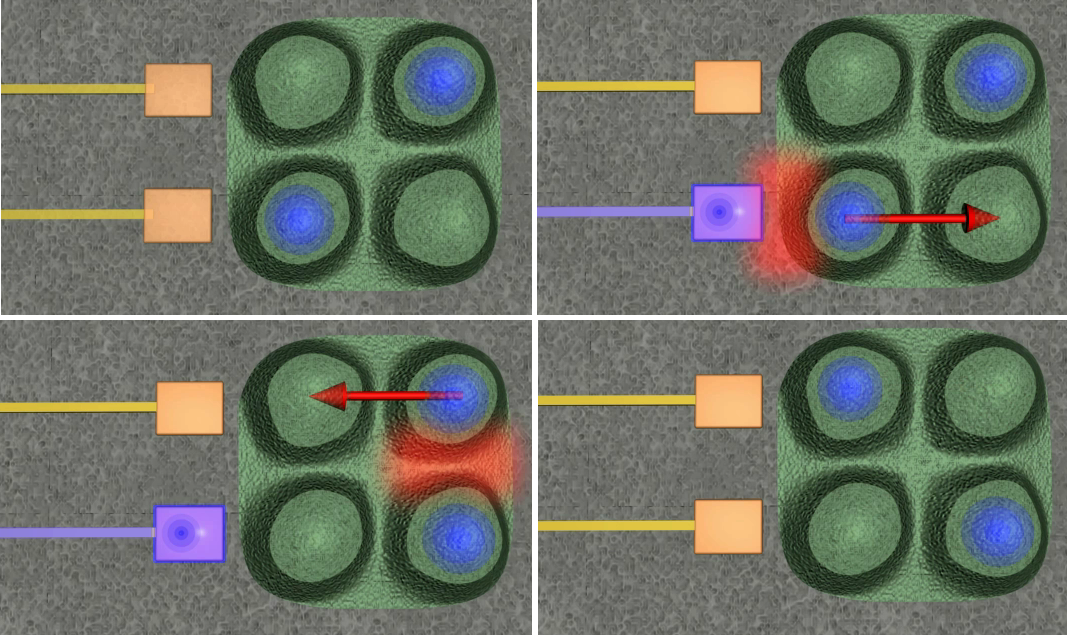
\includegraphics[width=0.9\textwidth]{img/qcaevo.png}}
	\caption{The evolution of the state of a QCA cell. From left to right, from top to bottom: the lower of the two wires (on the left in every image) is polarized, inducing (second image) the lower left electron to flow to the righest side of the QCA (and precisely inside the corresponding well). This, in turn, induces the upper right electron to move farthest from it, inside the upper left well (third and fourth image).}
	\label{fig:qcaevo}
\end{figure}

As an example of a QCA cells based circuit it is reported in Figure \ref{fig:qcamaj}. The conjunction of adjacent electrical fields of the three input drivers results into the polarization

\begin{figure}[h!bt]
	\centerline{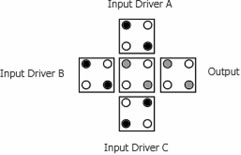
\includegraphics{img/qcamaj.png}}
	\caption{The majority gate drives the output cell's state to be equal to that of the majority of the inputs.}
	\label{fig:qcamaj}
\end{figure}

Apart from the possibility of using QCA for building quantum computing, which is something quite not at hand yet, QCAs can be seen as a powerful alternatives to silicon-based devices to represent data. Depending on the fabrication technique employed, in fact, QCAs are theorethically able to switch at an order of magnitude around the Thz, to be packaged at very high density levels and to disspate very small amounts of power. This, along with the existance of demo systems already proven working, justifies their current and future development as an attractive way of improving nowadays computing performance bottlenecks.

One of the universities interested and involved into the development of this technology, among the others, is the University of Columbia, and in particular its Microsystems and Nanotechnology Group (MiNa Group). The foundation of our work is their implementation of a simulator (both logical and physical) of QCA based cicuits and is the subject of the next section.



\newpage
\chapter{Cuda Overview}\label{sec:i}
Cuda is a software layer that allow programmers to exploit the capability of Nvidia GPUs as general purpose processors.\\
Dealing with a video card in this way requires approaching a completely new programming style and acquiring some knowledge about the basic Nvidia GPUs architectures, even though all the internal details are masked by the framework.\\
%First of all, as a philosophical remark, a GPU cannot run anything conceived and written for a CPU, as every vector stream architecture. In order to product software that can be executed on a Cuda Capable GPU, the programmer must write natively parallel code using one of the supported languages, extended with ad hoc Cuda primitives. There is no tool that can perform automatic porting of a sequential code into a parallel one.\\
Cuda exposes the GPU as a "Parallel Co-Processor" that can be used by the CPU to speed-up the computations. More in detail, the CPU - Host - can take advantage of the high amount of parallel threads executable by the GPU - Device - to accellerate parts of a program that are specially well suitted to exploit TLP. According to this, the CPU must directly manage the program execution settings on the GPU, provide the data for the computation to the device and collect the outputs when it has done.\\
One of the most important feature of Cuda is that it abstracts away all the physical details of the supported GPUs and shows to the programmer always the very same logical organization (Figure 3.1). These GPUs can be considered a MIMD array of SIMD processors, called MultiProcessors. Each MultiProcessor is mainly composed by 3 logic elements: a fixed number of cores, an instruction unit and a private memory space. All the MultiProcessors share a pubblic memory space referred to as Device Memory in order to distinguish it from the CPU memory space - Host Memory - that is not directly accessed by the GPU. Due to the property of abstraction mentioned before, the only difference between families of Nvidia products is in the amount of memory, the number of MultiProcessor and the nature of the cores.\\

\begin{figure}[h!bt]
	\centerline{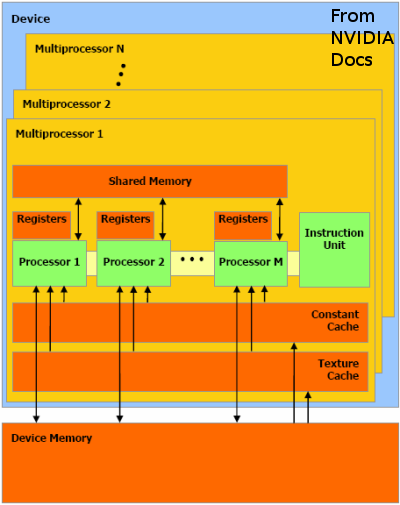
\includegraphics[width=0.5\textwidth]{img/HWModel.png}}
	\caption{Logical Organization of all the Cuda capable devices. The programmer does not have to take care of the physical organization of the GPU that will actually execute the program.}
	\label{fig:NvidiaGPUsLogicalOrg}
\end{figure}

\section{Multiprocessors}
Even if the architectural details on the Cuda capable GPU can significantly differ from a product to another, some common guidelines can be identified. The computational units of these GPUs are designed to be as simple and fast as possible. In order to keep low the complexity of the MPs, there are no branch predictors, nor any mechanisms to rollback incorrect results. Even if this can seems a serious limitation to the performance, it allow the cores of the MP to be completely focused on the arithmetic intensity. As results of this choice, the MP of the most recent Nvidia products are able to perform a double precision MAD (or MUL or ADD) per clock cycle.\\

\section{Memory Hierarchy}
The Cuda memory hierarchy consists of several elements optimized for different memory usages.\\
The Device Memory is the main memory space of the Video Card. It can be accessed by both the CPU and the GPU using different policies, usually with a latency of some hundred of clock cycles. In order to avoid confusion, it is logically partitioned into three logic component, depending on the access method: the Global Memory, that follow the common 32-,64-, or 128-byte memory transactions paradigm; Texture Memory, accessed by texture fetching; Constant Memory, managed by special operations.\\
The Global Memory is the most frequently employed memory space. Usually it is used by the CPU to load the data for the computations into the device and by the GPU to provide the results. Furthermore the Global Memory is the only space completely shared among all the SPs of the defice, for this reason it is also exploited for comunication among SPs belonging to different MPs. The Texture Memory can be written by the CPU using the Cuda API and readed by the GPU via texture fetching. No GPU texture write mechanism is provided. The Constant memory is a small special memory space that can be used for allocation of variables frequently readed. These variables must be allocated by the CPU before the execution on GPU, that can access them only in read-mode.\\ 
Due to the high latency of the Device Memory, each MP is provided of a private low latency memory space, logically composed by: a so called Shared Memory, directly accessible by all the SPs of the MP; a Constant Cache and a Texture Cache, managed by the framework; a set of exclusive Registers for each SP.\\
The Shared Memory can be considered as both a sort of cache of the Global Memory directly administrated by the cores in the MP and a mechanism for comunications among SPs belonging to the same MP. The Constant Cache and the Texture Cache are L1 caches used to speed-up the access time of the Constant Memory and the Texture Memory respectively. Due to the fact that Constant Memory and Texture Memory are read-only from the point of view of the GPU, no cache coherency protocol is needed.\\ 

\section{Programming Model}
As stated at the beginning of this chapter, the Cuda framework enable the programmer to take advantage of the high number of parallel threads executable by the GPU to expoit TLP: ideally the program is organized into identical sub-problems - working on different data - that can be solved independently. Each of this sub-problems, called Kernel, is mapped into a thread that will be executed on a SP.\\
All the threads executed by the SPs of a single MP are logically organized into a structure called Block. Virtually all the Threads belonging to a Block are execuded in parallel. Actually the number of SPs in a MP is usually much less than the number of Threads in a Block, for this reason only a part of the Threads is in concurrent execution at a given time, the so called Warp. When a MP is charged of a Block, it partitions this into warp that get sheduled by a warp sheduler for the execution on that MP. Due to the fact that all the Threads of a Block are executed on the same MP, it should be noticed that they share all the MP resources (i.e. Shared Memory and Caches) and that they can be synchronized using a specific API barrier.\\
All the Blocks are groupped into another logical structure called Grid. Considering that the number of Blocks of the Grid is usually greater than the numper of MPs, not all the Blocks can be sheduled at the same time. Since the blocks are unordered, they can execute equally well on a GPU that can handle one block at a time and one that executes a dozen or a hundred at a time, as demonstration of the scalability offered by the framework. In order to avoid complicating the Block scheduling process, no extra-block threads syncronization mechanism is provided.\\ 

\begin{figure}[h!bt]
	\centerline{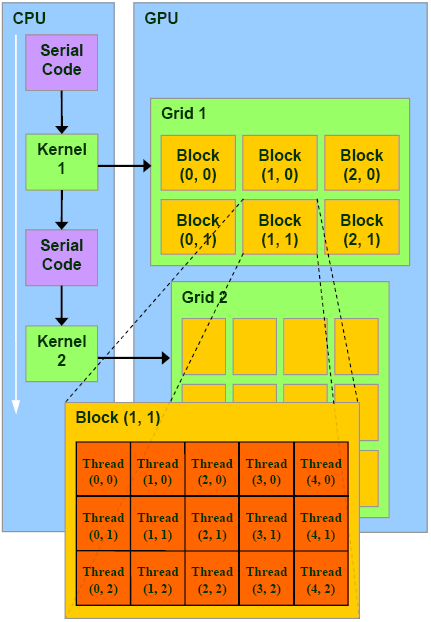
\includegraphics[width=0.5\textwidth]{img/NvidiaExecutionModel.png}}
	\caption{Nvidia Execution Model, an example of eterogeneous programming.}
	\label{fig:NvidiaGPUsLogicalOrg}
\end{figure}

\section{Best Pratices}



\newpage
\chapter{Implementation}\label{sec:implementation}
\section {The original tool}
The original tool is a Graphical Integrated Development Environment called QCADesigner, which is both meant for easing the process of layouting a QCA cells based circuit and for simplyfing the process of simulation and collection of the results. The layout view allows to place on the virtual PCB any number of QCA cell and defining if it is an input, output or fixed one. This discrimination makes it possible for the system to understand of which cells it is meaningful to record the polarization (the output cells) and to which one it is meaningful to assign a value (the input cells). Two different ways of simulating the behaviour of the circuit are implemented: the Coherence Vector and the Bistable engines. 

Both realize the abstract notion of Cellular Automata: the status of every cell at a given instant $t$ strictly depends on its state and on that of its neighborhood at $t-1$. The reason why two engines exist is quite simple: Bistable simulates the behaviour of the circuit from a ''logical'' point of view, meaning that it basically ''switches'' the polarization of every cell based on the polarization of the neighborhood and the current clock in \textsl{just one step}. Coherence Vector, instead, calculates at each instant $t$ the current polarization of the cell and that of its neighborhood and integrates over time the differential equations describing this system in order to make it evolve. Their authors compare and contrast these two engines this way: ''...It is believed that although this approximation [that of Bistable engine] is sufficient to verify the logical functionality of a design it cannot be extended to include valid dynamic simulation; but, as a result of its simplicity this simulation engine is able to simulate a large number of cells very rapidly, and therefore provides a good in-process check of the design. For dynamical simulations refer to the coherence vector simulation. ''. A few number of parameters allow for the customization of the behaviour of both engines in order to make the simulation as accurate and fast as possible. A few rules of thumb are available on the web site of the MiNa Group in order to effectively set some of them.

In the original implementation, moreover, it is possible to look at the evolution of the polarization of every cell during the simulation process.
\section {The bottlenecks of the original implementation}
First of all let's make a basic asymptotic analysis of the implementation of the Coherence Vector algorithm: we have $n$ cells that can have an average of $b$ neighbours. The engine basically runs trough every cell (this goes as $O(n)$) in the design and compute the current polarization based on the polarization of the previous step of all the neighbours (this goes as $O(b)$), and this is done for any possible combination of the inputs (this goes as $O(2^i)$). That is an asymptotic time complexity of $O(2^i*n*b)$  (worst case: $b$=$n-1$) and a space complexity of $O(n)$ (only the vector of the polarizations of every cell must be saved, anything else is computed using these values).

Now, the main bottleneck of the original implementation derives from the \textsl{serialization} of the simulation of a system that could be actually evolved \textsl{in parallel}, both with respect to $i$ (eg: one thread per configuration of the inputs) and with respect to $n$ (eg: one thread per cell per iteration). The original simulation of the system in this serial fashion, moreover, introduces some additive error (even though distributable over all cells randomizing the order in which they are simulated at each iteration) due to an overlapping of the writes related to different time instants. 

Our focus is set, in particular, on the Coherence Vector engine. The evidence of the limitations of the bottlenecks, here, are more evident than in Bistable because there is not not even the stabilization phase that would require additional costly synchronization mechanism/convergence criteria at each iteration of the simulation. In Coherence Vector mode the system is always free to evolve.

Before starting talking about the improved version it is good to remember that a number of runs of a set of test circuits has been made with QCADesigner in order to establish the baseline for the evaluation of the progresses (measured in seconds necessary to run the entrire simulation).
\section {Parallelization in CUDA}
\subsection{The approach}
The guiding idea during the parallelization process is: any cell in the system evolves independently with respect to the evolution of the other cells at the same time, but only on the previous state of the machine. Moreover, any input configuration is totally independent on every other possible configuration. In line of principle, this could be approached in one (or both) of these two ways:
\begin{itemize}
\item parallelize with respect to $i$: spread the computation of all the possible $2^i$ configuration on that many threads.
\item parallelize with respect to $n$: spread the computation of all the cells belonging to the same iteration on that many threads.
\end{itemize}
Our choice has been to follow the latter approach, mainly because 
\begin{itemize}
\item major limiting factor of the former approach: it is feasible only for combinatoric circuits; sequential ones still need to consider the variation of the inputs in order to determine their dynamic. Simulating a sequential circuit by means of a single input is practically useless.
\item the "one cell-one thread" approach is easy both to figure out and to manage
\item parallelizing with respect to the number of inputs would make the single kernel \textsl{very} complex, disallowing a number of possible optimizations (eg:occupancy improvement, branch divergence)  
\item not the very same actions should be taken for every cell at any moment of the simulation of different inputs; this introduces a hurdle in terms of branch divergence that doesn't allow the GPU to fully exploit its resources
\item suppose to be simulating $k$ configurations of the inputs at a time. The spatial complexity of the algorithm increases by $k$ (which grows exponentially with the number of inputs!).
\end{itemize} 

Moreover, the second approach allows us to better exploit the SIMD principle proper of all CUDA enabled devices because inside the same iteration of the simulation the actions to be carried over any cells are quite the same (and those cells who are not complying with this general scheme don't induce particularly critic divergences in the kernel). This approach allows for the same instructions to be concurrently executed on different data. In our particular case, the code basically does the same actions of the original implementation, apart from the details regarding the proper distribution of the computation among the available resources.

Last but not least, no \textsl{tile-problem} exists (the problem of overlapping adjacent concurrently simulated areas of circuit) because every single cell evolves independently of the effects of the neighbours at the \textsl{same} time $t$.

\subsection{The implementation}
Now, the datils of the implementation.

\begin{figure}[h!]
	\begin{center}$
		\begin{array}{cc}
			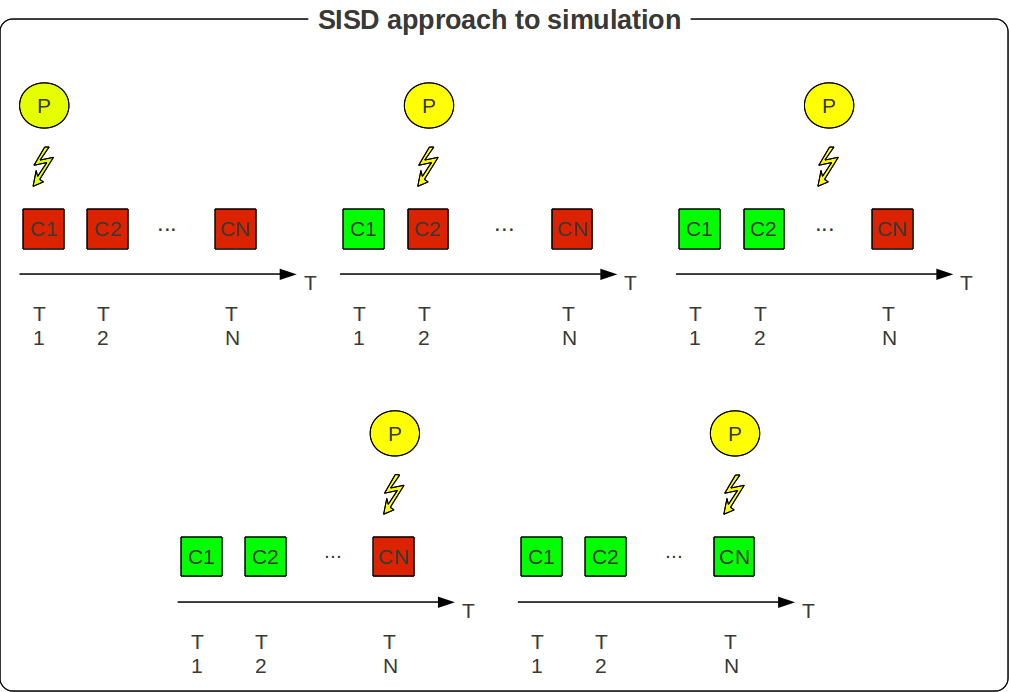
\includegraphics[width=0.5\textwidth]{img/impdetsisd.png} &
			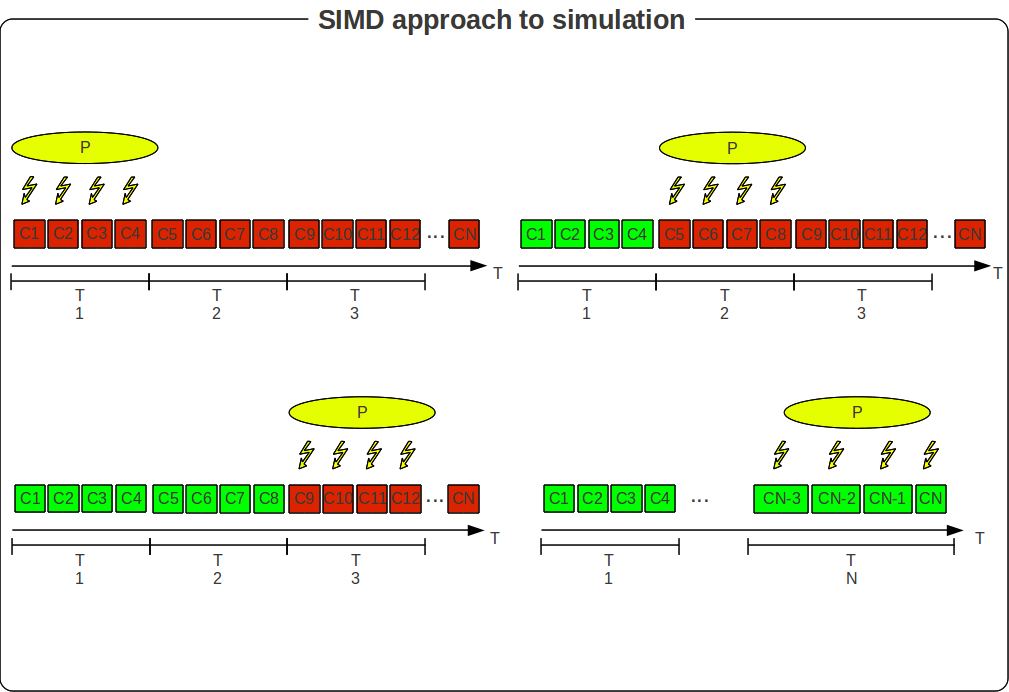
\includegraphics[width=0.5\textwidth]{img/impdetsimd}
		\end{array}$
	\end{center}
	\caption{\label{fig:impdet}In the first approach (SISD) each cell is evolved into the new state \textsl{one at a time}. Observing that any cell inside the same iteration can be evolved \textsl{in parallel} allows us to exploit a SIMD architecture in order to replicate the same instructions over a large number of cells at a time.}
\end{figure}

After an initial phase of parsing the command line commands, the flow of the program goes into Bistable or Coherence Vector engine.

In Coherence Vector mode, three different things happen.

First, all the useful data structures are initialized (for the output, for the parameters of the solver, for the iteration over all the cells into the design, notably). Among the others, some structures we had to implement in order to ease the process of converting the orignal data to CUDA compatible ones. In particular, we extract the following data:
\begin{itemize}
\item \textsl{polariztion vector} the vector of the initial polarization of every cell  (size: $n$)
\item \textsl{neighbour matrix} the unique index associated to every cell is found in this vector in position $i$ if and only if that cell is a neighbour of cell of uinique identifier $i$  (size: $n*b$)
\item \textsl{clock value} a value between 0 to 3 representing the phase of the clock (size: $n$)
\item \textsl{kink energy matrix} the element in position x,y contains the double representing the kink energy between element x and element y, and it is fixed troughout the whole simulation. (size: $n*b$)
\item \textsl{next polarization vector} each element of this matrix represents the evolution of the state of the corresponding cell and is computed by an apposite kernel function (size: $n$)
\end{itemize}
These data are represented in Figure \ref{fig:impdetmem}

\begin{figure}[h!bt]
	\centerline{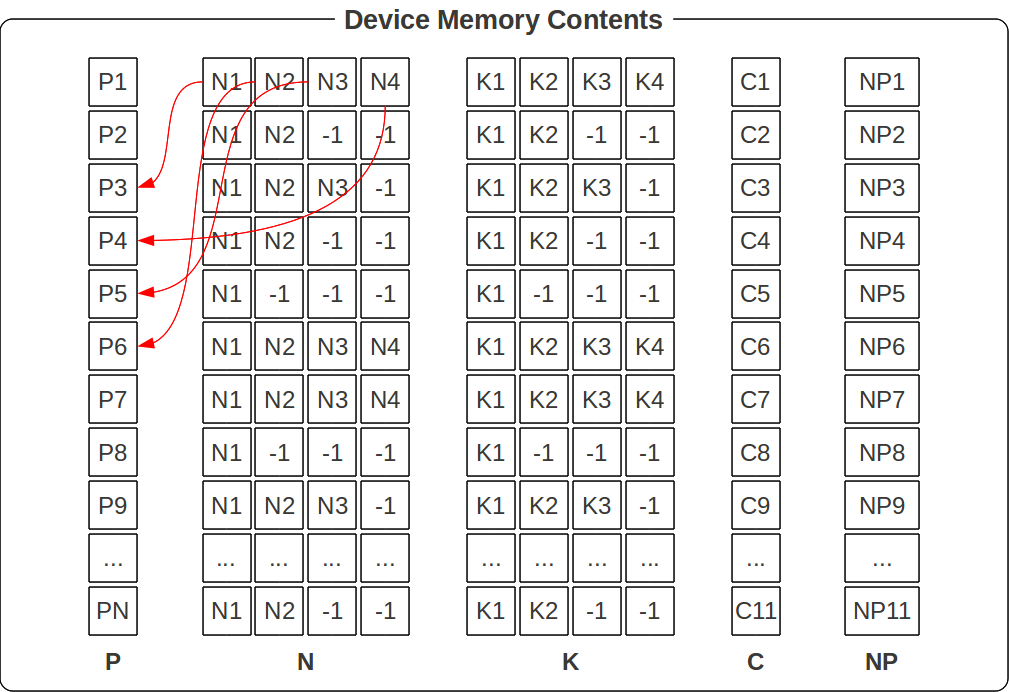
\includegraphics[width=0.8\textwidth]{img/impdetmem.png}}
	\caption{The contents of the memory. \textbf{P} and \textbf{NP} are, respectively, the vector of current polarization and the vector of next/future polarization. \textbf{N} is the matrix containing the ''pointers'' (in red) to the neighboring cells. A $-1$ in any position means that there are no more neighbours. This is because not all the cells must have the same number of neighbors and the matrix must have fixed dimensions while no value can be left unset. \textbf{K} matrix, instead, represent the kink energy that is instaurated between the corresponding neighbouring cells. \textbf{C} vector contains the clock value (the pahse of) for the corresponding cell.}
	\label{fig:impdetmem}
\end{figure}

Second, a number of calls to the framework APIs are made in order to load all the necessary data to the GPU. During this phase the geometry of the blocks of threads is also defined.

Third, the main iteration begins its execution. This loop is executed $f$ times, one for each instant required to completely simulate all the possible combinations of the inputs with the given time sampling (which is indeed a parameter settable via the command line). During each of the $f$ iterations all the $n$ cells in the design are evolved. This is basically the same happening in the serial code with the exception that we are capable of launching \textsl{one thread per cell}, each of which is able to calculate autonomously the evolution of the cell and storing this result in the corresponding cell of the \textbf{NP} vector (refer to Figure \ref{fig:impdetmem}). 

This part of the algorithm is the core of the speedup of our solution. What we do here, in contrast with the SISD approach of the original version of Coherence Vector, is exploiting a SIMD architecture in order to run $T$ (truly parallel) threads computing the evolution of $T$ different cells at once, without compromising the correctness of the simulation.

At the end of each iteration, the \textbf{NP} vector is transferred back from device to host memory and the polarization values written back into the original structures in order to be further treated, for example for saving to the output structures. These steps could have been (partly) done in GPU, but the cost\slash benefit ratio has been estimated too high to be convenient improving this part of the code. After this phase, the iteration goes to instant $t+1$, the polarizations are loaded into device memory and the evolution kernel is launched once again.

Our approcach, moreover, reduces the overall simulation error with respect to the CPU one: in fact, the evolution of the single cell in CPU mode is directly overwritten inside the \textsl{current} state, thus leading to the undesired effect of computing the state of the neighbour of $x$ with a polarization value that is already the future one. This is a limitation known to the MiNa Group who preferred to save execution time (otherwise to be dedicated to costly memory allocations/deallocations) in favour of a slightly more imprecise simulation.

After these improvements, the complexity of the algorithm changes in the following way. From a time perspective we have a theorethical speedup by $T$ running threads; in reality it is slightly less due to the inveitable serializations of the threads concurrently accessing the polarizations of common neighbors in the \textbf{P} vector and only under the assumption that the ratio (time spent loading data to/from device/host)/(time spent simulating the circuit inside the GPU) is negligible. This is similar to what happens with loop unrolling + software pipelining. From a space perspective, instead, we obtain (refer to Figure \ref{fig:impdetmem}) a complexity of $O(3*n+2*n*b)=O(n(3+2*b))$ (worst case: $b=n-1$).
\subsection{Optimizations}
A number of optimizations have been taken into account for improving the overall performance of the program.
\begin{itemize}
\item \textsl{memory hierarchy exploitation} memory in CUDA is higly hierarchical. Global memory is the main and largest memory pool of the device, at the cost of the slowest access speed. For this reason, whenever possible, it has been tried to move data to constant memory (e.g. all the optimization dependent constant values, pre calculated ones etc). No shared memory can be effectively shared between threads because the neighbours of a cell are not necessarily the same neighbours of another thread in the same warp. Other examined solutions comprised more or less huge (read: low speed) transfers of data from host to device memory, impacting at once both on the size of the largest possible simulated circuit and a huge amount of overhead not justified by a proportional in-kernel time. For example, instead of passing the uinique identifiers to the neighboring cells (the \textbf{N} matrix) one could directly pass the \textsl{value} of their polarization, allowing, for example, easier coalescent accesses. Even though, at first, this approach could be positively judged, at a deeper inspection it results in a predictable failure. In fact, every time the iteration ends we are required to exit from the kernel and overwrite the old polarization values with the new ones, thus \textsl{invalidating} the matrix passed just the step before. Our estimate is that a transfer of $n*b$ more doubles (64bit each in CUDA) at each iteration would impose a strong penalty to those circuits that are particulary well suited for simulation in GPU, \textsl{id} est the big ones.
\item \textsl{register usage} registers in CUDA capable devices are a scarce resource that directly and strongly impact the overall performance of a kernel. In fact, the number of threads \textsl{truly} concurrently running depends on how many registers are available inside the streaming multiprocessor to support their execution. Even though it is possible to define what is the optimal geometry of the running blocks by hand, nVidia made available a simple spreadsheet that allows for a fast computation of the optimal parameters for the particular kernel running on the particular system. The term ''occupancy'' in this context refers to the efficiency at exploiting the resources and is defined, more precisely, as the ratio of active warps to the maximum number of warps supported on a multiprocessor of the GPU. Obviously, the higher the occupancy, the higher the active warps, the faster the computation. In order to improve the occupancy factor we developed two different versions of the main kernel, one for each type of integration method employed fo the evolution of the polarization of the cells. This allowed us to reduce at once both the complexity of the single kernel (reducing the number of branches and the total number of instructions) as well as the number of registers required to run them (from 20 to 16, each 64 bits wide).
This is actually the best ppossible solution under a Tesla C1060 (the actual card used for testing purposes), yelding, in fact, a 100\% occupancy rate.
\item \textsl{exploitation of fast\_math} CUDA capable devices do not fully comply to the IEEE754 standard for floating point, double precision operations in that they allow a bigger ulp error for certain operations, in particular for trigonometric ones. In particular, the absolute value of the difference in ulps between a correctly rounded double-precision result and the result returned by the CUDA library function is 2 for cosine and 1 for the hyperbolic tangent. In our code we largely make use of floating point operations, so, by Amdhal's law, it is a good place where to look for improvements. One of those could be the demoting of the double arguments to float ones, in order to exploit the fast\_math mode of the CUDA C math library. In this mode, cosine function and division operation take only one clock cycle to execute, allowing for the highest possible troughput under this architecture. [noi non l'abbiamo ancora provata, potrebbe essere interessante ma nn abbiamo tempo per testarla - la mettiamo? la mettiamo come possibile ma non testata per motivi di tempo?]
\item \textsl{small transfers of data to/from host/device memory} these are by far the slowest possible operations that must be limited as much as possible. Our solution requires the lowest number of transfers among the proposed ones.
\item \textsl{coalescent access to (global) memory} the property of \textsl{coalescent} access to a memory location, in CUDA, holds iif any access from any thread happens to a memory bank not being read by any another different thread. This property allows the threads to simultaneously read to these different locations of memory without behing serialized. In our implementation we \textsl{did not} exploit coalescent accesses because of the peculiar geometry and interdependance of the data loaded into device memory that made it difficult (not possible) to figure out an efficient way of enabling this feature. 
\end{itemize}


\newpage
\chapter{Results}\label{sec:results}


\newpage
\chapter{Conclusions}\label{sec:conclusions}
possibility of implementing the vector table schema
possibility of further testings on clusters of tesla



%============================= BIBLIOGRAPHY =================================

\newpage

%this is the standard for bibliography references for IEEE Transactions	
\bibliographystyle{settings/IEEEtran}
\bibliography{DocBibliography}

\end{document}
